\documentclass[a4paper, 14 pt, titlepage]{extarticle}

\usepackage{grffile}
\usepackage{cmap}					% поиск в PDF
\usepackage[english,russian]{babel}	% локализация и переносы
\usepackage{indentfirst} 
\frenchspacing
\usepackage{setspace}
\usepackage{fontspec}      %% подготавливает загрузку шрифтов Open Type, True Type и др.
\defaultfontfeatures{Ligatures={TeX},Renderer=Basic}  %% свойства шрифтов по умолчанию
\setmainfont[Ligatures={TeX,Historic}]{Times New Roman} 
\setmonofont{Courier New}

\usepackage{amsmath,amsfonts,amssymb} 
\usepackage{amsthm}
\usepackage{mathtools}
\usepackage{icomma}

\renewcommand{\epsilon}{\ensuremath{\varepsilon}}
\renewcommand{\phi}{\ensuremath{\varphi}}
\renewcommand{\kappa}{\ensuremath{\varkappa}}
\renewcommand{\le}{\ensuremath{\leqslant}}
\renewcommand{\leq}{\ensuremath{\leqslant}}
\renewcommand{\ge}{\ensuremath{\geqslant}}
\renewcommand{\geq}{\ensuremath{\geqslant}}
\renewcommand{\emptyset}{\varnothing}
\newcommand{\eps}{\ensuremath{\varepsilon}}

\usepackage[unicode, pdfencoding=auto]{hyperref}
\usepackage[usenames,dvipsnames,svgnames,table,rgb]{xcolor}
\hypersetup{
            unicode=true,
            colorlinks=true,
            linkcolor=black,
            urlcolor=blue
           }

\usepackage{graphicx}
\graphicspath{{images/}}
\usepackage{wrapfig}
\usepackage{tikz}

\usepackage{array,tabularx,tabulary,booktabs, longtable, multirow}

\usepackage{etoolbox}
\usepackage{caption}
\captionsetup{labelsep=endash, font={singlespacing}, figurename=Рисунок }

\usepackage{fancyhdr} % Колонтитулы
 	\pagestyle{fancy}
 	\renewcommand{\headrulewidth}{0pt}  % Толщина линейки сверху
    \fancyfoot[R]{\thepage}
    \fancyfoot[C]{}
    \fancyhead[R]{}
    
\setstretch{1.5}

\usepackage{extsizes}
\usepackage{geometry}
\geometry{top=2cm}
\geometry{bottom=2cm}
\geometry{left=3cm}
\geometry{right=1.5cm}

\usepackage{listings}
\usepackage{color}

\lstset{
	basicstyle=\footnotesize\ttfamily,
	tabsize=4,
	columns=fixed,
	extendedchars=true,
	lineskip=-0.05\baselineskip,
	aboveskip=6pt,
	belowskip=6pt,
	breaklines,
	showstringspaces
}

\renewcommand{\thesection}{\Asbuk{section}}

\usepackage{titlesec}
\titleformat{\section}{\centering\normalsize\normalfont\bfseries}{}{0ex}{ПРИЛОЖЕНИЕ \thesection\\\uppercase}{}

\titleformat{\subsection}{\normalsize \normalfont \bfseries}{\thesubsection}{}{}
\titlespacing\subsection{1.25cm}{1cm}{0pt}

\parindent=1.25cm

\newcommand{\startcode}{
    \footnotesize
    \singlespacing
}

\newcommand{\finishcode}{\setstretch{1.5}\normalsize}

\newenvironment{code}{\startcode}{\finishcode}

\newcommand{\printcaption}[1]{
    \normalsize
    {
    \captionsetup{justification=raggedright, singlelinecheck=off}
    \caption{#1}
    }
}


\newcommand{\subject}{Параллельные алгоритмы}
\newcommand{\labnumber}{5}
\newcommand{\teacher}{Сергеева~Е.И.}
\newcommand{\theme}{Знакомство с программированием гетерогенных систем в стандарте Open CL}
\newcommand{\name}{Эйсвальд~М.И.}

\setlength{\extrarowheight}{1mm}

\begin{document}

\begin{titlepage}
   
   \begin{center}
       {\onehalfspacing
        \textbf{
             МИНОБРНАУКИ РОССИИ\\
             САНКТ-ПЕТЕРБУРГСКИЙ
             ГОСУДАРСТВЕННЫЙ
             ЭЛЕКТРОТЕХНИЧЕСКИЙ
             УНИВЕРСИТЕТ <<ЛЭТИ>> ИМ.~
             В.И.~УЛЬЯНОВА (ЛЕНИНА)\\
            Кафедра МО ЭВМ\\
            \vspace{7cm}
            ОТЧЁТ\\
            по лабораторной работе №\labnumber\\
            по дисциплине <<\subject>>\\
            Тема: \theme\\
        }
        
        \vspace{5cm}
        %\vspace{2.0cm}
        
       
       
       \setlength{\extrarowheight}{4mm}
       \begin{tabulary}{\textwidth}{LCCCL}
            Студент гр. 9303 & \hspace{0.5cm} & \hspace{4.5cm} & \hspace{0.5cm} & \name \\
            \cline{3-3}
            Преподаватель & \hspace{0.5cm} & \hspace{4.5cm} & \hspace{0.5cm} & \teacher \\
            \cline{3-3}
       \end{tabulary}
       \setlength{\extrarowheight}{0mm}
       
       \vfill
       
       Санкт-Петербург\\
       \the\year\\
       }
       
   \end{center}
   
  \end{titlepage}




\setcounter{page}{2}

\subsection*{Цель работы.}
Получить навыки работы в стандарте OpenCL, изучить возможности стандарта OpenCL.

\subsection*{Выполнение работы.}

За основу работы было взято опубликованное в репозитории демонстрационное приложение, использующее OpenCL. Приложение засекает время, затраченное на нахождение приближения множества Мандельброта на заданном количестве пикселей с заданным числом итераций, после чего находит приближение множества Мандельброта на каждом устройстве компьютера, поддерживающем стандарт OpenCL, также засекая затраченное время. Результат вычислений с помощью OpenCL сохраняется в виде PNG-изображения с помощью сторонней библиотеки. Пример изображения представлен на рисунке ниже.

\begin{figure}[!h]
	\centering
	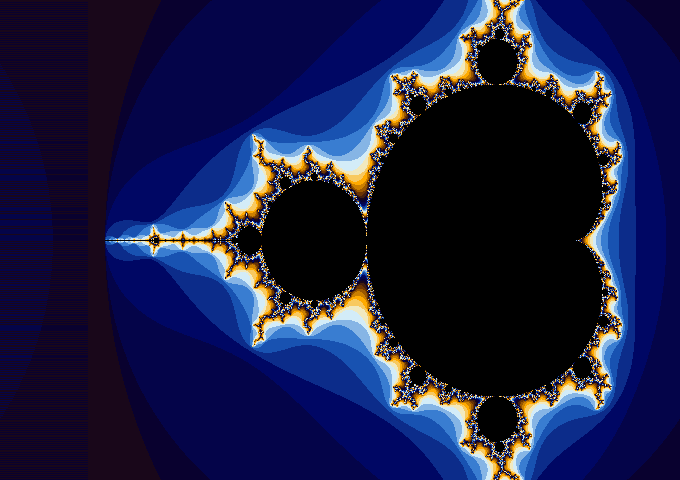
\includegraphics[width=\linewidth]{output}
	\caption{Визуализация приближения множества Мандельброта}
\end{figure}

Сравнение производительности последовательных вычислений и вычислений с помощью OpenCL представлено в таблице ниже.

\begin{table}[!h]
	\centering
	\begin{tabulary}{\textwidth}{|C|C|C|C|}
		\hline
		Размер изображения, пикселей&Количество итераций&Время работы итеративного алгоритма, мс&Время работы алгоритма на основе OpenCL, мс\\\hline
		680$\times$480&10&13&1\\\hline
		680$\times$480&50&34&2\\\hline
		680$\times$480&100&58&2\\\hline
		680$\times$480&1000&479&13\\\hline
		680$\times$480&10000&4640&106\\\hline
		800$\times$600&10&19&2\\\hline
		800$\times$600&50&50&3\\\hline
		800$\times$600&100&86&3\\\hline
		800$\times$600&1000&708&22\\\hline
		800$\times$600&10000&6789&151\\\hline
	\end{tabulary}
\end{table}

\subsection*{Выводы.}
В ходе выполнения работы были изучены основы работы со стандартом OpenCL. Было установлено, что скорость работы OpenCL-приложений над хорошо распараллеливаемой задачей на порядки превышает скорость работы итеративных решений. Результатом работы стало приложение, визуализирующее фрактал Мандельброта.

%\newpage
%\section{Демонстрация процесса создания цифровой подписи ECDSA}

\end{document}
